\documentclass[11pt,compress,t,notes=noshow, xcolor=table]{beamer}
\usepackage[]{graphicx}\usepackage[]{color}
% maxwidth is the original width if it is less than linewidth
% otherwise use linewidth (to make sure the graphics do not exceed the margin)
\makeatletter
\def\maxwidth{ %
  \ifdim\Gin@nat@width>\linewidth
    \linewidth
  \else
    \Gin@nat@width
  \fi
}
\makeatother

\newcommand{\citebutton}[2]{%
\beamergotobutton{\href{#2}{#1}}%
}

\newcommand{\blu}[1]{\textcolor{blue}{#1}}
\newcommand{\org}[1]{\textcolor{orange}{#1}}
\newcommand{\ques}{\textbf{\textcolor{red}{Question:  }}}
\newcommand{\questionssofar}{\begin{frame}\frametitle{Any questions?}\end{frame}}

\newcommand\warning{%
 \makebox[1.4em][c]{%
 \makebox[0pt][c]{\raisebox{.1em}{\scriptsize!}}%
 \makebox[0pt][c]{\color{red}\normalsize$\bigtriangleup$}}}%

\definecolor{fgcolor}{rgb}{0.345, 0.345, 0.345}
\newcommand{\hlnum}[1]{\textcolor[rgb]{0.686,0.059,0.569}{#1}}%
\newcommand{\hlstr}[1]{\textcolor[rgb]{0.192,0.494,0.8}{#1}}%
\newcommand{\hlcom}[1]{\textcolor[rgb]{0.678,0.584,0.686}{\textit{#1}}}%
\newcommand{\hlopt}[1]{\textcolor[rgb]{0,0,0}{#1}}%
\newcommand{\hlstd}[1]{\textcolor[rgb]{0.345,0.345,0.345}{#1}}%
\newcommand{\hlkwa}[1]{\textcolor[rgb]{0.161,0.373,0.58}{\textbf{#1}}}%
\newcommand{\hlkwb}[1]{\textcolor[rgb]{0.69,0.353,0.396}{#1}}%
\newcommand{\hlkwc}[1]{\textcolor[rgb]{0.333,0.667,0.333}{#1}}%
\newcommand{\hlkwd}[1]{\textcolor[rgb]{0.737,0.353,0.396}{\textbf{#1}}}%
\let\hlipl\hlkwb

\usepackage{framed}
\makeatletter
\newenvironment{kframe}{%
 \def\at@end@of@kframe{}%
 \ifinner\ifhmode%
  \def\at@end@of@kframe{\end{minipage}}%
  \begin{minipage}{\columnwidth}%
 \fi\fi%
 \def\FrameCommand##1{\hskip\@totalleftmargin \hskip-\fboxsep
 \colorbox{shadecolor}{##1}\hskip-\fboxsep
     % There is no \\@totalrightmargin, so:
     \hskip-\linewidth \hskip-\@totalleftmargin \hskip\columnwidth}%
 \MakeFramed {\advance\hsize-\width
   \@totalleftmargin\z@ \linewidth\hsize
   \@setminipage}}%
 {\par\unskip\endMakeFramed%
 \at@end@of@kframe}
\makeatother

\definecolor{shadecolor}{rgb}{.97, .97, .97}
\definecolor{messagecolor}{rgb}{0, 0, 0}
\definecolor{warningcolor}{rgb}{1, 0, 1}
\definecolor{errorcolor}{rgb}{1, 0, 0}
\newenvironment{knitrout}{}{} % an empty environment to be redefined in TeX

\usepackage{alltt}
\newcommand{\SweaveOpts}[1]{}  % do not interfere with LaTeX
\newcommand{\SweaveInput}[1]{} % because they are not real TeX commands
\newcommand{\Sexpr}[1]{}       % will only be parsed by R
\newcommand{\xmark}{\ding{55}}%


\usepackage[english]{babel}
\usepackage[utf8]{inputenc}

\usepackage{dsfont}
\usepackage{verbatim}
\usepackage{amsmath}
\usepackage{amsfonts}
\usepackage{amssymb}
\usepackage{bm}
\usepackage{csquotes}
\usepackage{multirow}
\usepackage{longtable}
\usepackage{booktabs}
\usepackage{enumerate}
\usepackage[absolute,overlay]{textpos}
\usepackage{psfrag}
\usepackage{algorithm}
\usepackage{algpseudocode}
\usepackage{eqnarray}
\usepackage{arydshln}
\usepackage{tabularx}
\usepackage{placeins}
\usepackage{tikz}
\usepackage{setspace}
\usepackage{colortbl}
\usepackage{mathtools}
\usepackage{wrapfig}
\usepackage{bm}
\usepackage{amsmath}
\usepackage{pifont}

\usetikzlibrary{shapes.multipart,shapes,arrows,automata,positioning,calc,chains,trees, shadows}
\tikzset{
  %Define standard arrow tip
  >=stealth',
  %Define style for boxes
  punkt/.style={
    rectangle,
    rounded corners,
    draw=black, very thick,
    text width=6.5em,
    minimum height=2em,
    text centered},
  % Define arrow style
  pil/.style={
    ->,
    thick,
    shorten <=2pt,
    shorten >=2pt,}
}

\tikzstyle{vec}=[draw, rectangle, fill = white, minimum width=5mm, minimum height=1cm, inner sep = 2pt]

\usepackage{subfig}

% Defines macros and environments
\usepackage{../../style/lmu-lecture}


\let\code=\texttt
\let\proglang=\textsf

\setkeys{Gin}{width=0.9\textwidth}

\setbeamertemplate{frametitle}{\expandafter\uppercase\expandafter\insertframetitle}

\usepackage{bbm}
% basic latex stuff
\newcommand{\pkg}[1]{{\fontseries{b}\selectfont #1}} %fontstyle for R packages
\newcommand{\lz}{\vspace{0.5cm}} %vertical space
\newcommand{\dlz}{\vspace{1cm}} %double vertical space
\newcommand{\oneliner}[1] % Oneliner for important statements
{\begin{block}{}\begin{center}\begin{Large}#1\end{Large}\end{center}\end{block}}


%new environments
\newenvironment{vbframe}  %frame with breaks and verbatim
{
 \begin{frame}[containsverbatim,allowframebreaks]
}
{
\end{frame}
}

\newenvironment{vframe}  %frame with verbatim without breaks (to avoid numbering one slided frames)
{
 \begin{frame}[containsverbatim]
}
{
\end{frame}
}

\newenvironment{blocki}[1]   % itemize block
{
 \begin{block}{#1}\begin{itemize}
}
{
\end{itemize}\end{block}
}

\newenvironment{fragileframe}[2]{  %fragile frame with framebreaks
\begin{frame}[allowframebreaks, fragile, environment = fragileframe]
\frametitle{#1}
#2}
{\end{frame}}


\newcommand{\myframe}[2]{  %short for frame with framebreaks
\begin{frame}[allowframebreaks]
\frametitle{#1}
#2
\end{frame}}

\newcommand{\remark}[1]{
  \textbf{Remark:} #1
}


\newenvironment{deleteframe}
{
\begingroup
\usebackgroundtemplate{
\includegraphics[width=\paperwidth,height=\paperheight]{../style/color/red.png}}
 \begin{frame}
}
{
\end{frame}
\endgroup
}
\newenvironment{simplifyframe}
{
\begingroup
\usebackgroundtemplate{
\includegraphics[width=\paperwidth,height=\paperheight]{../style/color/yellow.png}}
 \begin{frame}
}
{
\end{frame}
\endgroup
}\newenvironment{draftframe}
{
\begingroup
\usebackgroundtemplate{
\includegraphics[width=\paperwidth,height=\paperheight]{../style/color/green.jpg}}
 \begin{frame}
}
{
\end{frame}
\endgroup
}
% https://tex.stackexchange.com/a/261480: textcolor that works in mathmode
\makeatletter
\renewcommand*{\@textcolor}[3]{%
  \protect\leavevmode
  \begingroup
    \color#1{#2}#3%
  \endgroup
}
\makeatother





\input{../../latex-math/basic-math.tex}
\input{../../latex-math/basic-ml.tex}
\usepackage{movie15}
\usepackage{animate}

\newcommand{\titlefigure}{figure/sesamestreet.jpeg}
\newcommand{\learninggoals}{
\item reformulating classification tasks
\item multi-task learning
\item fine-tuning on task-prefixes}

\title{Post-BERT Era}
% \author{}
\institute{\href{https://slds-lmu.github.io/lecture_dl4nlp/}{slds-lmu.github.io/lecture\_dl4nlp}}
\date{}

\begin{document}
\lecturechapter{Tasks as text-to-text problem}
\lecture{Deep Learning for NLP}

% ------------------------------------------------------------------------------

\begin{frame}{Recap: BERT, RoBERTa, etc.}

\vfill

  \begin{itemize}
\item Transformer encoder
\item Training: Masked language modeling (or similar)
\item BERT* learns an enormous amount of knowledge
about language and the world through MLM training on large corpora
\item Application: fine-tune on a particular task
\item Great performance!
\item \ques What's not to like?
    \end{itemize}

\vfill

*\scriptsize{In what follows we will use BERT as a representative for this class of language models, i.e. models with a custom classification layer of each task, and only talk about BERT -- but the discussion includes RoBERTa, Albert, XLNet etc.}

\end{frame}

% ------------------------------------------------------------------------------

\begin{frame}{Problems with BERT (1)}

\vfill

  \begin{itemize}
\item You need a different model for each task.
\item[] (Because BERT is differently fine-tuned for each task.)
\item[] $\to$ Not realistic in many real deployment scenarios, e.g., on mobile devices.
\item \textit{Human learning:} We arguably have a \myblue{single} model that solves all tasks!
\item \ques Is there a framework that allows us to create a single model that solves all tasks?
    \end{itemize}

\vfill

\end{frame}

% ------------------------------------------------------------------------------

\begin{frame}{Problems with BERT (2)}

\vfill
			
\begin{itemize}
\item Two training modes: first (MLM) pretraining, then fine-tuning.
\item Fine-tuning is \myblue{supervised learning}, i.e., learning from labeled examples.
\item Arguably, learning from labeled examples is untypical for human learning.
\item You never learn a task solely by being presented a bunch of examples, without explanation.
\item Instead, in human learning, there is almost always a \myblue{task description}.
    \end{itemize}

\vfill

\end{frame}

% ------------------------------------------------------------------------------

\begin{frame}{Problems with BERT (2)}

\vfill
			
\begin{itemize}
\item Example: \textit{How to boil an egg.}
		\begin{itemize}
			\item ``Place eggs in the bottom of a saucepan.``
			\item ``Fill the pan with cold water.``
			\item ``Etc.``
		\end{itemize}
\item Notice that this is \myblue{not} an example but a \textit{description} of the task
\item \ques Is there a framework that allows us to leverage task descriptions?
\end{itemize}

\vfill

\end{frame}

% ------------------------------------------------------------------------------

\begin{frame}{Problems with BERT (3)}

\vfill

  \begin{itemize}
\item BERT has great performance, but \ldots
\item \ldots only if the training set is large, generally 1000s of examples
\item This is completely different from human learning!
\item We do use examples in learning, but in most cases, only a few
\end{itemize}

\vfill

\end{frame}

% ------------------------------------------------------------------------------

\begin{frame}{Problems with BERT (3)}

\vfill

  \begin{itemize}
\item Example: Maybe the person teaching you how to boil an egg will show you how to do it \textit{one or two times}
\item But probably \myblue{not} 10 times
\item Definitely \myblue{not} a 1000 times 
\item More practical concern: it's very expensive to label 1000s of examples for each task (there are many tasks).
\item \ques Is there a framework that allows us to learn from just a small number of examples?
\item This is called \myblue{few-shot learning}.
    \end{itemize}

\vfill

\end{frame}

% ------------------------------------------------------------------------------

\begin{frame}{Problems with BERT (4)}

\vfill

  \begin{itemize}
		\item More subtle aspect of the same problem (i.e., large training sets):
		\item[] $\to$ \textbf{Overfitting}
		\item Even though performance looks good on standard train/dev/test splits, the deviation between the training set and the
data actually encountered in real application can be large
		\item So our benchmarks often overestimate what performance would be in reality
  \end{itemize}

\vfill

\end{frame}

% ------------------------------------------------------------------------------

\begin{frame}{Problems with BERT -- summary}

\vfill

  \begin{itemize}
		\item No true multitask learning
		\item Differs from the way humans learn
		\item No possibility/necessity to make use of a description of the task
		\item Overfitting
  \end{itemize}

\vfill

\end{frame}

% ------------------------------------------------------------------------------

\begin{frame}{revisiting text-to-text tasks}

\vfill

\textbf{Example: Machine Translation}
	
	\begin{figure}
		\centering
		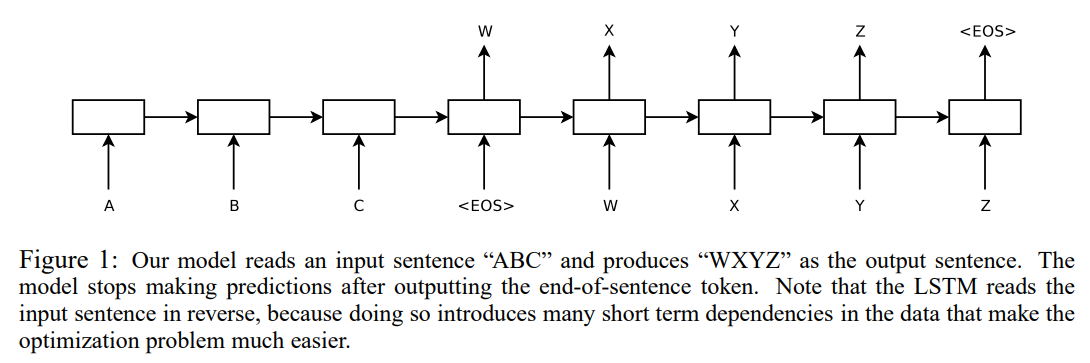
\includegraphics[width = 11cm]{../chapter01-basics/figure/seq2seq.png}\\ 
	\citebutton{Source: Sutskever et al., 2014}{https://arxiv.org/pdf/1409.3215.pdf}
	\end{figure}

\begin{itemize}
	\item \textit{Input:} Text in source language
	\item \textit{Output:} Text in target language
\end{itemize}

\vfill

\end{frame}

% ------------------------------------------------------------------------------

\begin{frame}{revisiting fine-tuning of bert}

\vfill

	\begin{figure}
	\centering
		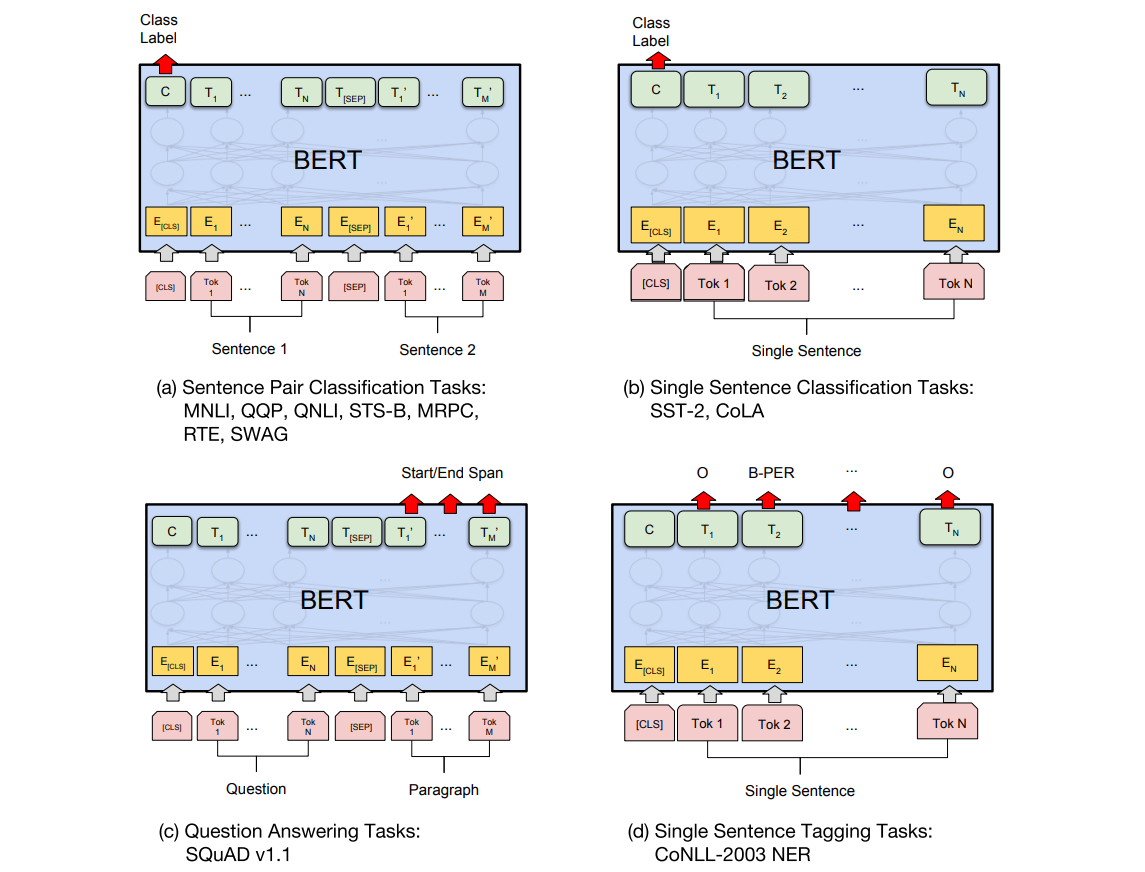
\includegraphics[width = 8cm]{../chapter04-bert/figure/bert-finetune.png}\\ 
	\citebutton{Source: Devlin et al., 2019}{https://aclanthology.org/N19-1423.pdf}
	\end{figure}
	
\begin{itemize}
	\item \textit{First row:} (sequence-level) classification
	\item \textit{Second row:} sequence tagging = token-level classification
\end{itemize}

\vfill

\end{frame}

% ------------------------------------------------------------------------------

\begin{frame}{fine-tuning + text-to-text?}

\vfill

\begin{itemize}
	\item \ques How does BERT know which task it is performing?
			\begin{itemize}
				\item It doesn't!
				\item BERT just learns associations between text features and class distributions
				\item No meaningful internal representation of what ``class 3`` actually \textit{means}
				\item \textit{Input}: text; \textit{Output}: \texttt{[0 0 1 0 0 0]}
			\end{itemize}
	\item The fact that BERT does not ``understand`` what task it is actually performing is the reason why one copy is needed per task
\end{itemize}

\vfill

\end{frame}

% ------------------------------------------------------------------------------

\begin{frame}{fine-tuning + text-to-text?}

\vfill

\begin{itemize}
	\item \ques How could we ``inform`` our model about the task?
			\begin{itemize}
				\item Model takes text as an input and can process.
				\item Why not describe the task in natural language?
				\item \textit{Assumption:}\\
							Given the model sees 1000s of (inputs; ouput) pairs like ..
			\end{itemize}
\end{itemize}

		\begin{center}
				{\small
					(``\texttt{<task description>: <input sample>}`` ; ``\texttt{<class name>}``)
				}
		\end{center}
				
\begin{itemize}
			\item[]
			\begin{itemize}
				\item .. it will learn to associate ..
				\item[] $\to$ .. task descriptions to a set of class names
				\item[] $\to$ .. text features to class name distributions
			\end{itemize}
\end{itemize}

\vfill

\end{frame}

% ------------------------------------------------------------------------------

\begin{frame}{fine-tuning + text-to-text?}

\vfill

\begin{itemize}
	\item \ques How does a ``good`` task description look like?
			\begin{itemize}
				\item Remember: The idea is to have a model that learns to associate the task descriptions with a set of class names
				\item \textit{Class names:} 
				\item[] $\to$ Could be pretty new/exotic terms the model is not familiar with after pre-training
				\item[] $\to$ It will learn to output them during fine-tuning when ``triggered`` accordingly (i.e. with the right task description)
				\item \textit{Task descriptions:} 
				\item[] $\to$ Might be possible that the the model already saw some task descriptions during pre-training and has a meaningful representation for them.
				\item[] $\to$ On the other hand: Others might also be pretty new/exotic.
			\end{itemize}
\end{itemize}

\vfill

\end{frame}

% ------------------------------------------------------------------------------

\begin{frame}{fine-tuning + text-to-text?}

\vfill

For sentiment classification, I can just provide it with 1000s of training samples like 

		\begin{center}
				{\small
					(``\texttt{<sentiment classification>: <input sample>}`` ; ``\texttt{<positive/negative>}``)
				}
		\end{center}
		
The model will ..

\begin{itemize}
	\item .. utilize already present knowledge about the task description.
	\item .. learn to associate the task description precisely with this label set
\end{itemize}

\vfill

\end{frame}

% ------------------------------------------------------------------------------

\begin{frame}{fine-tuning + text-to-text?}

\vfill

\begin{itemize}
	\item \ques If I want the model to do sentiment classification, can I also just provide it with 1000s of training samples like 
\end{itemize}

		\begin{center}
				{\small
					(``\texttt{<khaleesi>: <input sample>}`` ; ``\texttt{<positive/negative>}``)
				}
		\end{center}
				
\begin{itemize}
	\item[] ? 
	\item[] (\textit{khaleesi}$^1$ just used as some random fantasy word here)
	\pause
	\item \textit{Intuition:} Yes! It basically does not matter, \textbf{as long as the model is fine-tuned on this data}$^2$
	\item Fine-tuning important for the model to pick up on this ``signal`` and output according text (corresponding the appropriate classes)
\end{itemize}

\vfill

$^1$\footnotesize{Khaleesi is a Dothraki title referring to the wife of the khal (cf. Game of Thrones).}\\
$^2$\footnotesize{Of course, using ``good`` task descriptions (as shown on the previous slide) that are also meaningful to human readers make more sense as the model might learn quicker because they diverge less from the pre-training distribution.}

\end{frame}

% ------------------------------------------------------------------------------

\begin{frame}{multi-task learning?}

\vfill

\begin{figure}
	\centering
		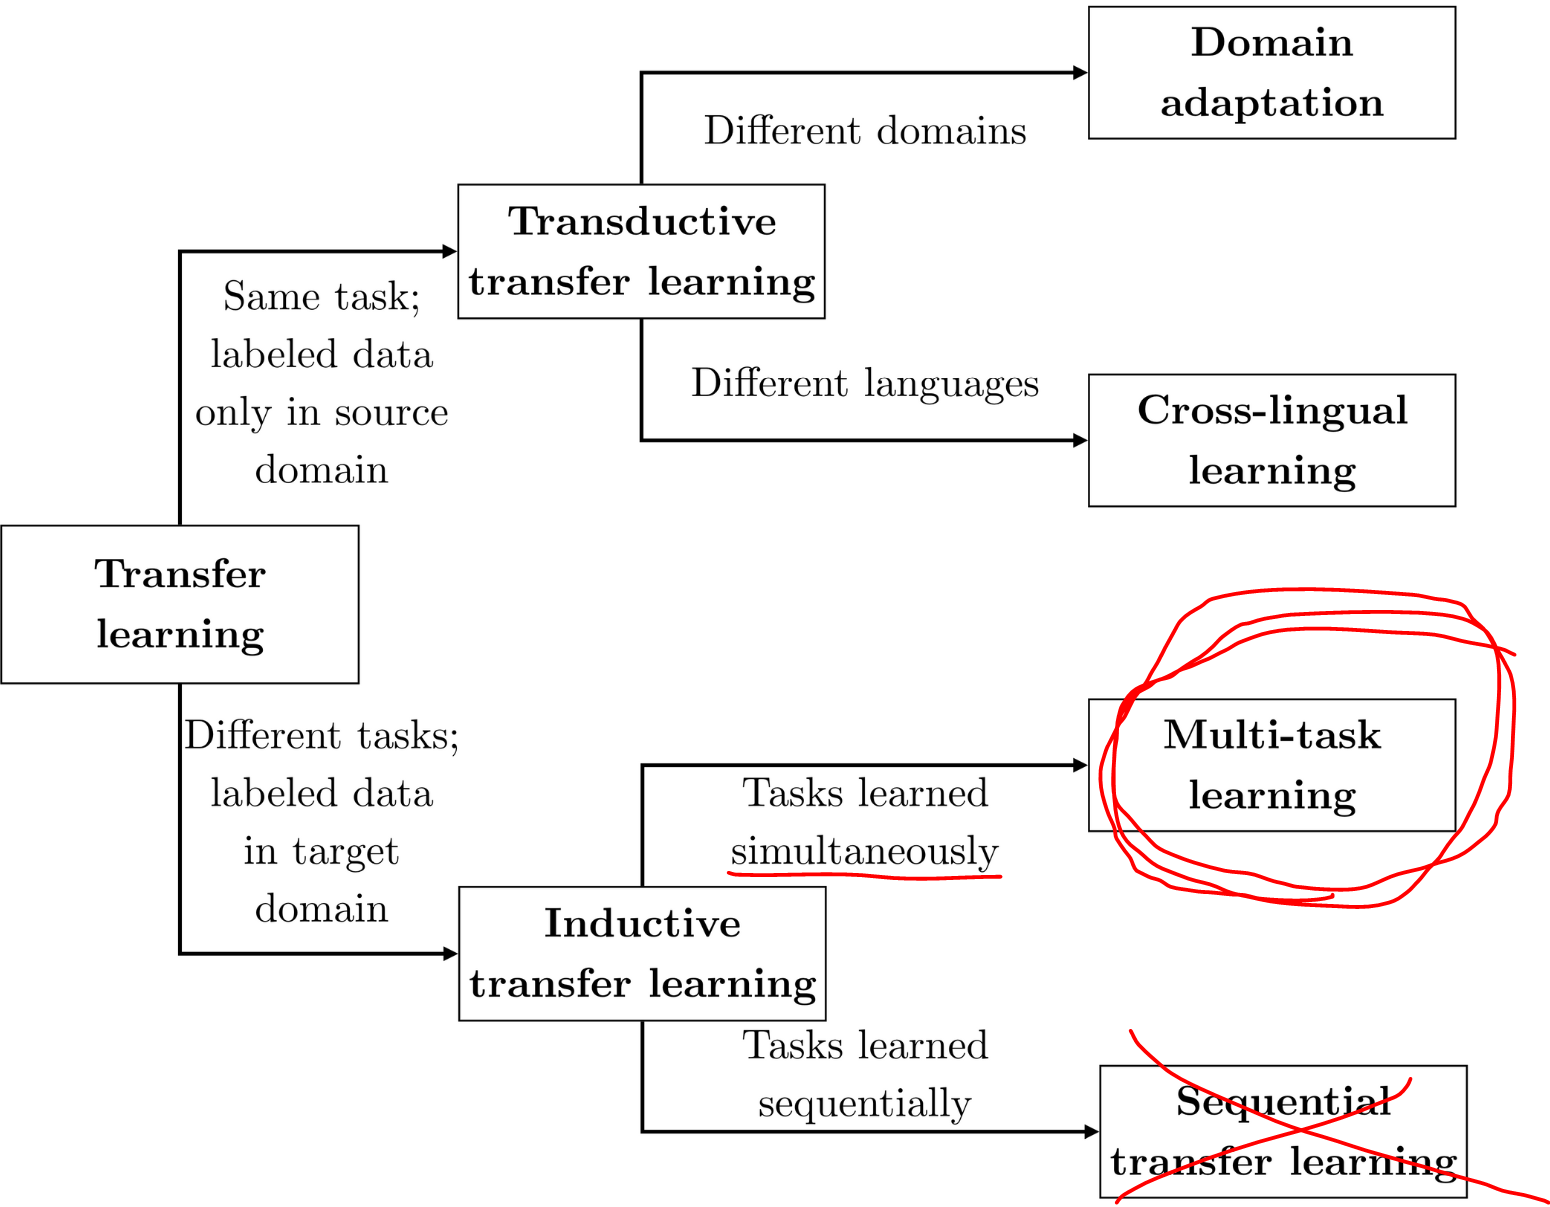
\includegraphics[width = 7cm]{figure/62-transfer_learning_taxonomy-anno.png}\\ 
	\beamergotobutton{Taxonomy of transfer learning \href{https://ruder.io/thesis/}{(Source: Ruder, 2019)}}
\end{figure}

\vfill

\end{frame}

% ------------------------------------------------------------------------------

\begin{frame}{multi-task learning?}

\vfill

\begin{itemize}
	\item \ques If the model can learn to link task descriptions to label sets, can it learn to perform multiple tasks at once?
	\item Yes, through fine tuning each task description$^1$ will be linked to its label set:
			\begin{itemize}
				\item \texttt{<task description a>} $\to$ \texttt{\{positive, negative\}}
				\item \texttt{<task description b>} $\to$ \texttt{\{world, sports, business, sci/tech\}} \citebutton{Example from AG News}{http://groups.di.unipi.it/~gulli/AG_corpus_of_news_articles.html}
				\item \texttt{<task description c>} $\to$ \texttt{\{spam, no spam\}}
				\item \texttt{<task description d>} $\to$ \texttt{\{entailment, contradiction, neutral\}}
			\end{itemize}
\end{itemize}

\vfill

$^1$\footnotesize{\texttt{<task description a>} (and so on) are just placeholders here.}
\end{frame}

% ------------------------------------------------------------------------------

\begin{frame}{multi-task learning?}

\vfill

\begin{itemize}
	\item \ques Can we have one single model for both different classification tasks \textbf{and} generation tasks?
			\begin{itemize}
				\item Yes, we just have to design suitable task descriptions
				\item Examples for \textit{generative} descriptions \citebutton{Raffel et al., 2020}{https://jmlr.org/papers/v21/20-074.html}
						\begin{itemize}
							\item \texttt{translate English to German: <input sample>}
							\item \texttt{summarize: <input sample>}
							\item \texttt{answer question: <input sample>}
						\end{itemize}
				\item Examples for \textit{classification} descriptions \citebutton{Raffel et al., 2020}{https://jmlr.org/papers/v21/20-074.html}
						\begin{itemize}
							\item \texttt{binary classification: <input sample>}
							\item \texttt{predict sentiment: <input sample>}
						\end{itemize}
			\end{itemize}
\end{itemize}

\vfill

\end{frame}

% ------------------------------------------------------------------------------

\begin{frame}{Text-to-Text Tasks}

\vfill
	
	\begin{figure}
		\centering
		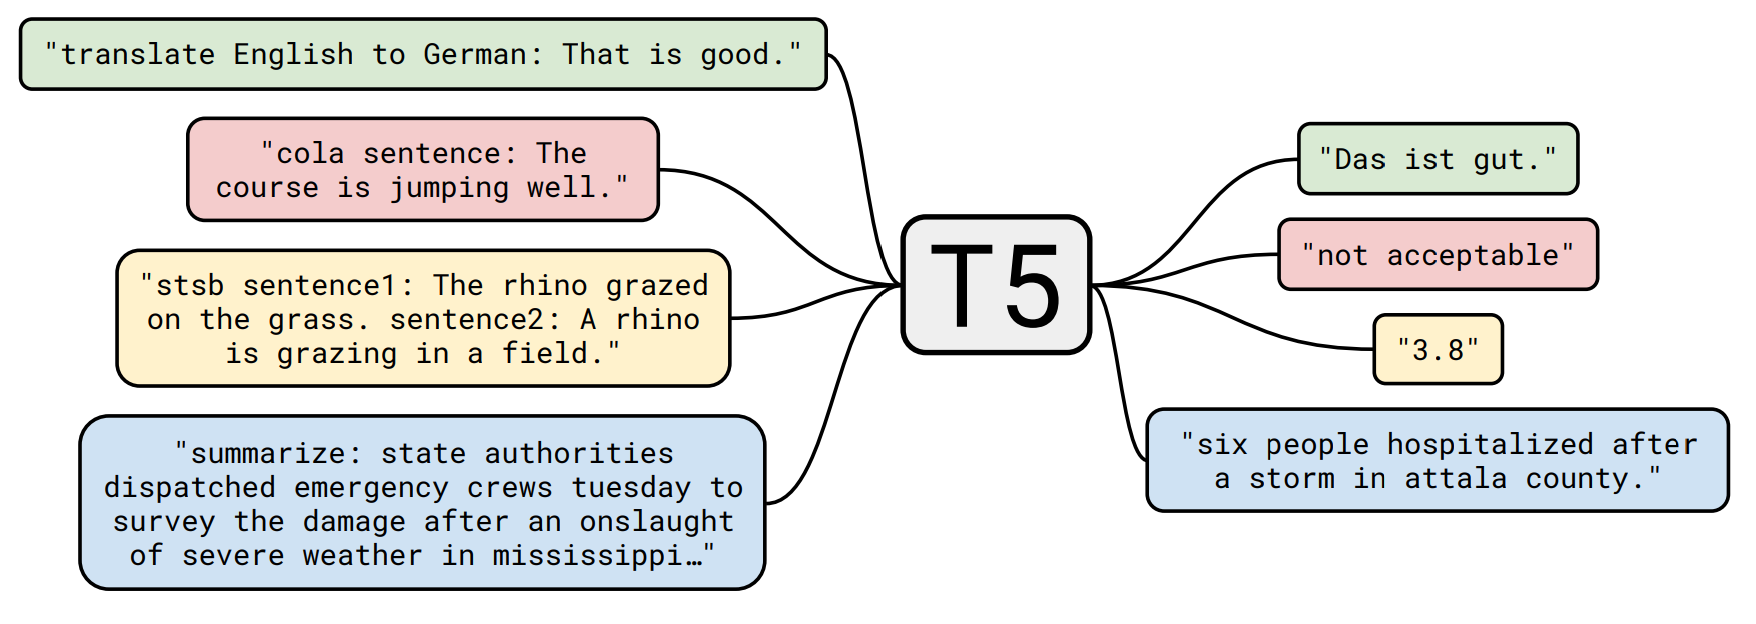
\includegraphics[width = 11cm]{figure/62-t5.png}\\ 
		\citebutton{Source: Raffel et al., 2020}{https://jmlr.org/papers/v21/20-074.html}
	\end{figure}
	
\begin{itemize}
	\item \textbf{Important note:} What we talked about as \texttt{<task description>} until now is commonly referred to as \texttt{<task prefix>}
\end{itemize}
	
\vfill

\end{frame}

% ------------------------------------------------------------------------------

\endlecture
\end{document}